\documentclass[14pt,a4paper]{extarticle}
% =============================================================
% preamble_compact.tex — компактный вариант оформления отчётов
% Основа — preamble.tex (СТП БГУИР); здесь только уплотнение:
% разделы без принудительного перехода на новую страницу,
% меньшие вертикальные отступы, плотные списки и подписи.
% =============================================================
% =============================================================
% preamble.tex — Shared LaTeX preamble for genetic/evolutionary reports
% Conforming to BSUIR STP 01-2024
% =============================================================

% Encoding and language
\usepackage[utf8]{inputenc}
\usepackage[T2A]{fontenc}
\usepackage[russian]{babel}

% Times New Roman font
\usepackage{tempora}

% Page geometry: STP 2.1.1
\usepackage{geometry}
\geometry{left=30mm, right=15mm, top=20mm, bottom=20mm}

% Line spacing: STP 2.1.1
\usepackage{setspace}
\singlespacing

% Allow TeX a bit more flexibility to avoid overflow
\pretolerance=1000
\tolerance=2000
\emergencystretch=3em

% Paragraph indent
\usepackage{indentfirst}
\setlength{\parindent}{1.25cm}

% Page numbers
\usepackage{fancyhdr}
\pagestyle{fancy}
\fancyhf{}
\fancyfoot[R]{\thepage}
\renewcommand{\headrulewidth}{0pt}
\fancypagestyle{plain}{%
  \fancyhf{}%
  \fancyfoot[R]{\thepage}%
  \renewcommand{\headrulewidth}{0pt}%
}

% Math
\usepackage{amsmath,amssymb}

% Graphics
\usepackage{graphicx}
\usepackage{float}
\usepackage{xcolor}

% Tables
\usepackage{booktabs}
\usepackage{tabularx}
\usepackage{multirow}
\usepackage{longtable}

% Captions
\usepackage{caption}
\captionsetup[figure]{
  labelsep=endash,
  justification=centering,
  font={normalsize},
  name=Рисунок
}
\captionsetup[table]{
  labelsep=endash,
  justification=raggedright,
  singlelinecheck=false,
  font={normalsize},
  name=Таблица
}

% Section formatting
\usepackage{titlesec}
\titleformat{\section}
  {\newpage\normalfont\fontsize{14}{18}\selectfont\bfseries}
  {\thesection}{0.5em}{\MakeUppercase}
\titlespacing*{\section}{1.25cm}{0pt}{14pt}

\titleformat{\subsection}
  {\normalfont\fontsize{14}{18}\selectfont\bfseries}
  {\thesubsection}{0.5em}{}
\titlespacing*{\subsection}{1.25cm}{14pt}{14pt}

\titleformat{\subsubsection}
  {\normalfont\fontsize{14}{18}\selectfont\bfseries}
  {\thesubsubsection}{0.5em}{}
\titlespacing*{\subsubsection}{1.25cm}{14pt}{14pt}

% Unnumbered sections
\newcommand{\sectioncenter}[1]{%
  \newpage
  \phantomsection
  \addcontentsline{toc}{section}{#1}
  \begin{center}
    \textbf{\MakeUppercase{#1}}
  \end{center}
  \vspace{14pt}
}

% Table of contents formatting
\usepackage{tocloft}
\renewcommand{\cftsecfont}{\normalfont}
\renewcommand{\cftsecpagefont}{\normalfont}
\renewcommand{\cftsubsecfont}{\normalfont}
\renewcommand{\cftsubsecpagefont}{\normalfont}
\renewcommand{\cftsecleader}{\cftdotfill{\cftdotsep}}
\renewcommand{\cftdotsep}{1}
\renewcommand{\contentsname}{\hfill\textbf{СОДЕРЖАНИЕ}\hfill}
\renewcommand{\cftaftertoctitle}{\hfill}

% Lists
\usepackage{enumitem}
\setlist[itemize]{noitemsep, topsep=0pt, leftmargin=1.25cm, label=--}
\setlist[enumerate]{noitemsep, topsep=0pt, leftmargin=1.25cm}

% Code listings
\usepackage{listings}
\usepackage{fancyvrb}
\lstset{
  basicstyle=\ttfamily\small,
  frame=single,
  breaklines=true,
  showstringspaces=false,
  inputencoding=utf8,
  extendedchars=true,
  literate={а}{{\cyra}}1 {б}{{\cyrb}}1 {в}{{\cyrv}}1 {г}{{\cyrg}}1
           {д}{{\cyrd}}1 {е}{{\cyre}}1 {ж}{{\cyrzh}}1 {з}{{\cyrz}}1
           {и}{{\cyri}}1 {й}{{\cyrishrt}}1 {к}{{\cyrk}}1 {л}{{\cyrl}}1
           {м}{{\cyrm}}1 {н}{{\cyrn}}1 {о}{{\cyro}}1 {п}{{\cyrp}}1
           {р}{{\cyrr}}1 {с}{{\cyrs}}1 {т}{{\cyrt}}1 {у}{{\cyru}}1
           {ф}{{\cyrf}}1 {х}{{\cyrh}}1 {ц}{{\cyrc}}1 {ч}{{\cyrch}}1
           {ш}{{\cyrsh}}1 {щ}{{\cyrshch}}1 {ъ}{{\cyrhrdsn}}1
           {ы}{{\cyrery}}1 {ь}{{\cyrsftsn}}1 {э}{{\cyrerev}}1
           {ю}{{\cyryu}}1 {я}{{\cyrya}}1
}

% Hyperlinks
\usepackage{hyperref}
\hypersetup{
  colorlinks=true,
  linkcolor=black,
  urlcolor=blue,
  citecolor=black,
}

% Number figures and tables within sections
\numberwithin{figure}{section}
\numberwithin{table}{section}
\numberwithin{equation}{section}

% Standard title page macro
\newcommand{\makegeclabtitle}[2]{%
  \begin{titlepage}
  \thispagestyle{empty}
  \begin{center}

  МИНИСТЕРСТВО ОБРАЗОВАНИЯ РЕСПУБЛИКИ БЕЛАРУСЬ

  \vspace{0.5em}

  Учреждение образования

  \vspace{0.5em}

  \textbf{<<Белорусский государственный университет информатики и радиоэлектроники>>}

  \vspace{2em}

  Факультет компьютерных систем и сетей

  \vspace{0.5em}

  Кафедра программного обеспечения информационных технологий

  \end{center}

  \vspace{3em}

  \begin{center}
  \textbf{ОТЧЕТ}

  \vspace{0.5em}

  по лабораторной работе №#1

  \vspace{0.5em}

  по дисциплине

  \vspace{0.5em}

  <<Генетические и эволюционные вычисления>>

  \vspace{0.5em}

  <<#2>>
  \end{center}

  \vspace{5em}

  \begin{flushright}
  \begin{minipage}{0.5\textwidth}
  \textbf{Выполнил:}\\
  Лебедевич Артем Владимирович\\
  магистрант группы 556301

  \vspace{0.6em}

  \textbf{Преподаватель:}\\
  Нестеренков Сергей Николаевич\\
  кандидат технических наук\\
  доцент кафедры ПОИТ
  \end{minipage}
  \end{flushright}

  \vfill

  \begin{center}
  Минск, 2026~г.
  \end{center}

  \end{titlepage}
}


% Разделы идут подряд, без \newpage
\titleformat{\section}
  {\normalfont\fontsize{14}{17}\selectfont\bfseries}
  {\thesection}{0.5em}{\MakeUppercase}
\titlespacing*{\section}{1.25cm}{12pt}{6pt}
\titlespacing*{\subsection}{1.25cm}{8pt}{4pt}

% Плотнее плавающие объекты и подписи
\setlength{\textfloatsep}{8pt plus 2pt minus 2pt}
\setlength{\floatsep}{6pt plus 2pt minus 2pt}
\setlength{\intextsep}{6pt plus 2pt minus 2pt}
\captionsetup[figure]{skip=3pt, font={small}}
\captionsetup[table]{skip=2pt, font={small}}
\setlength{\abovedisplayskip}{4pt}
\setlength{\belowdisplayskip}{4pt}

% Таблицы компактнее
\renewcommand{\arraystretch}{1.05}
\setlength{\tabcolsep}{5pt}

% Номера рисунков и таблиц — сквозные (без привязки к разделам)
\counterwithout{figure}{section}
\counterwithout{table}{section}
\counterwithout{equation}{section}

\graphicspath{{figures/}}

\begin{document}

\makegeclabtitle{7}{Генетические алгоритмы с вещественным и перестановочным представлением особей. Задача коммивояжёра}

\section{Цель работы}

Изучить представление особей в форме вещественных чисел и перестановок, специализированные генетические операторы для каждого представления и особенности решения задач непрерывной и комбинаторной оптимизации генетическими алгоритмами. Работа состоит из двух частей: А~--- ГА с вещественным кодированием для поиска минимума функции Растригина; Б~--- решение задачи коммивояжёра на наборе eil76 (TSPLIB) с циклическим кроссинговером (вариант~3).

\section{Краткие теоретические сведения}

\textbf{Вещественное кодирование.} Особь~--- вектор $\mathbf{x} \in \mathbb{R}^n$; ошибок дискретизации нет. BLX-$\alpha$ кроссинговер порождает ген потомка $c_i \sim U[\min(p_i^1, p_i^2) - \alpha d_i;\ \max(p_i^1, p_i^2) + \alpha d_i]$, $d_i = |p_i^1 - p_i^2|$. Гауссова мутация: $x_i' = x_i + \mathcal{N}(0, \sigma(t))$, где шаг $\sigma(t) = \sigma_0 (b - a)(1 - t/T)$ убывает~--- от исследования области к точной доводке. Тестовая функция Растригина:
\begin{equation}
f(x_1, x_2) = 20 + \sum_{i=1}^{2}\bigl[x_i^2 - 10\cos(2\pi x_i)\bigr], \quad x_i \in [-5{,}12;\ 5{,}12],
\end{equation}
имеет около 120 локальных минимумов в узлах целочисленной решётки и глобальный минимум $f(0, 0) = 0$.

\textbf{Задача коммивояжёра.} Требуется найти замкнутый маршрут минимальной длины, проходящий через все города по одному разу. При представлении путей тур~--- перестановка номеров городов. Циклический кроссинговер (CX) разбивает позиции на циклы соответствия родителей и берёт циклы попеременно: каждый город в потомке стоит на той же позиции, что и у одного из родителей. Мутация обменом (swap) меняет местами два города, инверсия переворачивает отрезок тура (заменяет два ребра). Локальный поиск 2-opt заменяет пару рёбер $(a, b), (c, d)$ на $(a, c), (b, d)$, пока это укорачивает тур.

\section{Часть А. ГА с вещественным кодированием}

ГА реализован на NumPy (\texttt{lab\_07.ipynb}): $N = 60$, турнир $k = 3$, BLX-0,5 с $P_c = 0{,}9$, гауссова мутация ($P_m = 0{,}2$ на ген, $\sigma_0 = 0{,}1$), две элитные особи. За 150 поколений (9\,060 вычислений функции) найден глобальный минимум с машинной точностью: $f = 0$, $|x_i| \sim 10^{-9}$. Уже к 10-му поколению популяция собирается в центральной <<яме>> (рисунок~\ref{fig:rast}).

\begin{figure}[H]
\centering
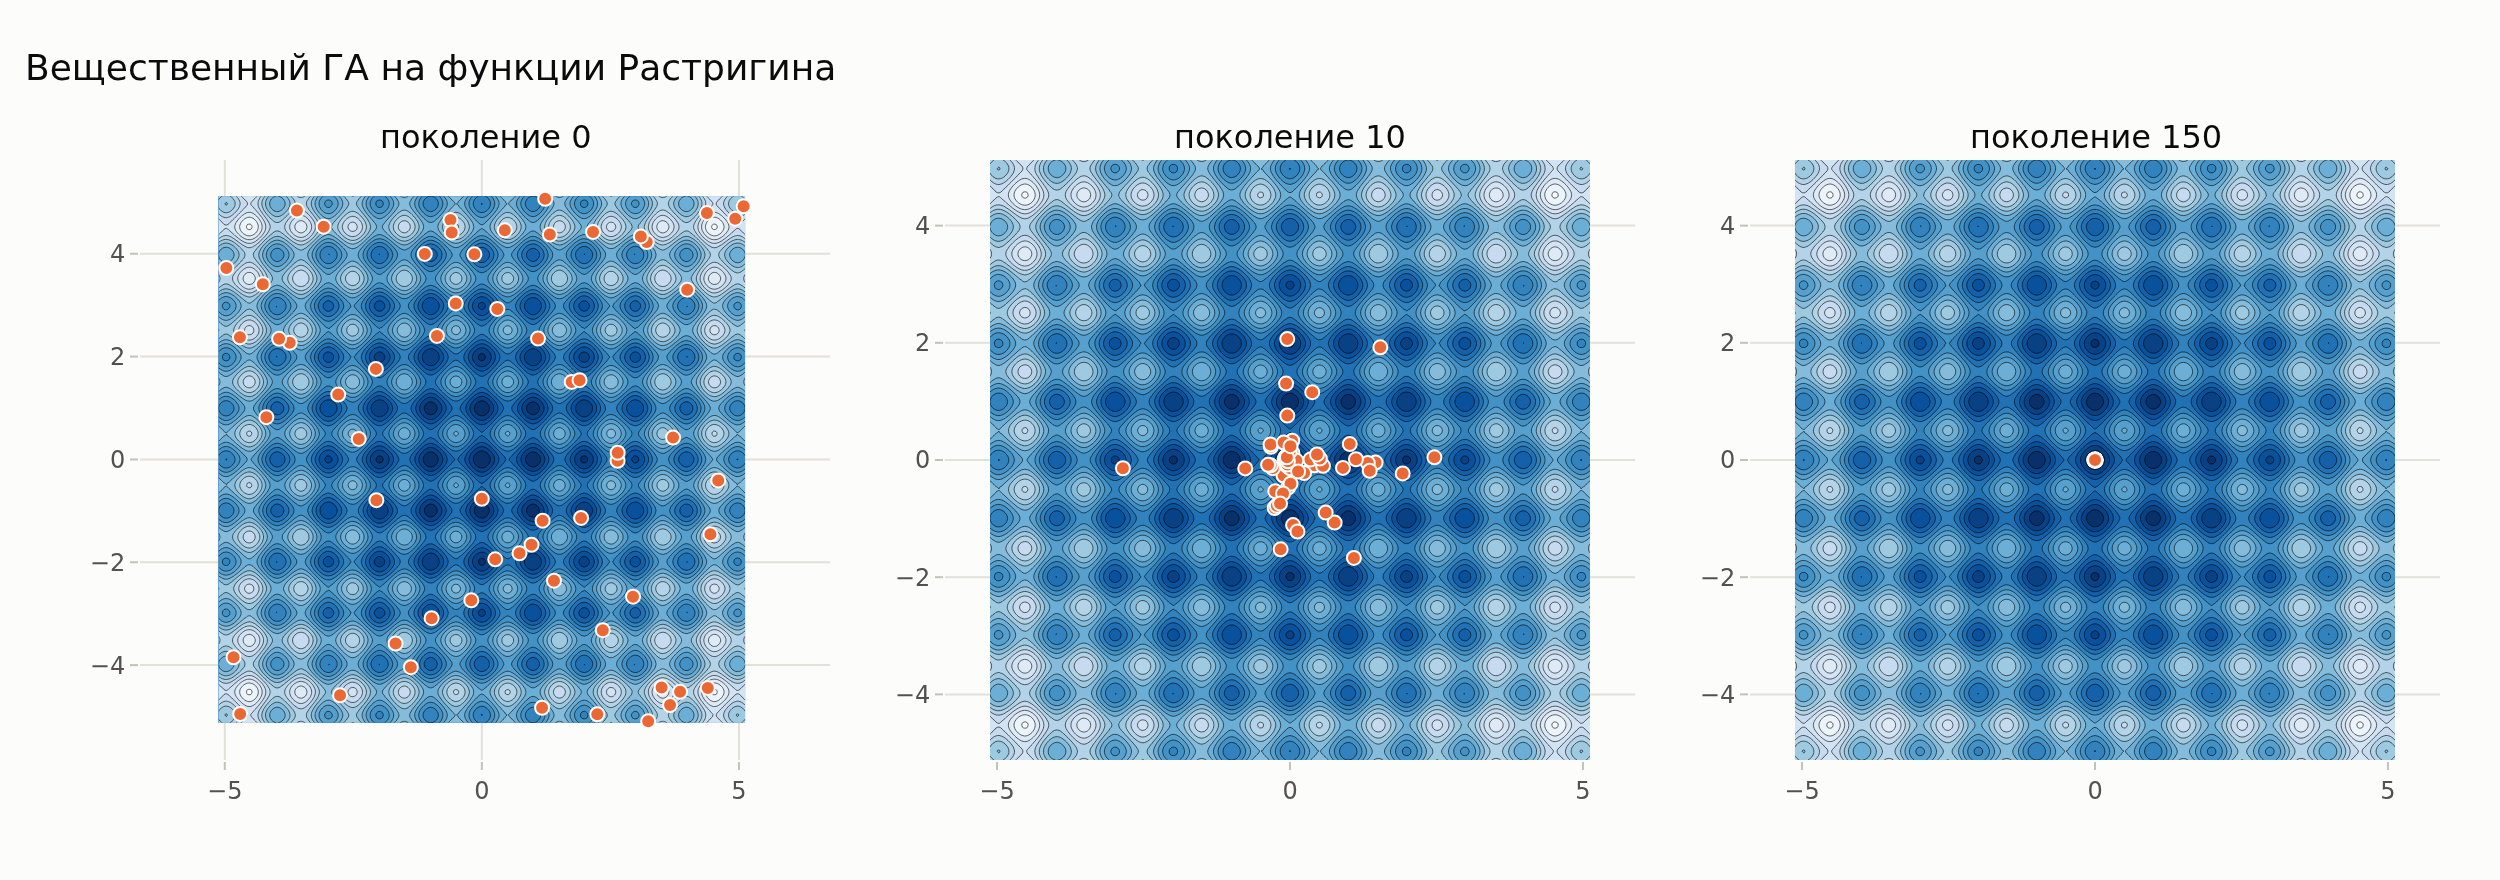
\includegraphics[width=\textwidth]{A1_population.png}
\caption{Популяция вещественного ГА на линиях уровня функции Растригина}
\label{fig:rast}
\end{figure}

\textbf{Параметры.} При 150 поколениях почти любая настройка находит минимум, поэтому параметры сравнивались при бюджете 50 поколений, по 20 запусков (успех~--- $f < 10^{-3}$, таблица~\ref{tab:realparams}).

\begin{table}[H]
\caption{Вещественный ГА на функции Растригина, 50 поколений (20 запусков на значение)}
\label{tab:realparams}
\centering
\small
\begin{tabular}{lcccc}
\toprule
Параметр & Значение & Медиана $f$ & Худшее $f$ & Успехов, \% \\
\midrule
параметр BLX-$\alpha$ & 0 & 6.5e-09 & 0.00 & 100 \\
параметр BLX-$\alpha$ & 0.25 & 1.8e-12 & 0.00 & 100 \\
параметр BLX-$\alpha$ & 0.5 & 2.1e-12 & 0.00 & 100 \\
параметр BLX-$\alpha$ & 1 & 2.6e-08 & 0.99 & 95 \\
шаг мутации $\sigma_0$ & 0 & 0.0e+00 & 0.99 & 80 \\
шаг мутации $\sigma_0$ & 0.02 & 2.8e-12 & 0.99 & 70 \\
шаг мутации $\sigma_0$ & 0.1 & 2.1e-12 & 0.00 & 100 \\
шаг мутации $\sigma_0$ & 0.3 & 7.5e-12 & 0.00 & 100 \\
вероятность мутации $P_m$ & 0 & 0.0e+00 & 0.99 & 80 \\
вероятность мутации $P_m$ & 0.05 & 0.0e+00 & 0.99 & 85 \\
вероятность мутации $P_m$ & 0.2 & 2.1e-12 & 0.00 & 100 \\
вероятность мутации $P_m$ & 0.5 & 2.6e-04 & 0.00 & 80 \\
размер популяции N & 20 & 8.6e-06 & 1.00 & 85 \\
размер популяции N & 40 & 2.3e-11 & 0.00 & 100 \\
размер популяции N & 60 & 2.1e-12 & 0.00 & 100 \\
размер популяции N & 120 & 5.9e-12 & 0.00 & 100 \\
\bottomrule
\end{tabular}
\end{table}


\textbf{Сравнение с бинарным кодированием.} Бинарный ГА из ЛР~№6 (20 бит на переменную) и вещественный ГА получили одинаковый бюджет $60 \times 150$ (таблица~\ref{tab:realbin}, рисунок~\ref{fig:realbin}).

\begin{table}[H]
\caption{Вещественное и бинарное кодирование при равном бюджете (20 запусков)}
\label{tab:realbin}
\centering
\small
\begin{tabular}{llccc}
\toprule
Функция & Кодирование & Медиана $f$ & Лучшее $f$ & Худшее $f$ \\
\midrule
Растригин & бинарное (20 бит) & 9.5e-09 & 9.5e-09 & 1.2e+00 \\
Растригин & вещественное & 0.0e+00 & 0.0e+00 & 4.6e-11 \\
Шаффер F7 & бинарное (20 бит) & 2.0e-02 & 2.0e-02 & 1.8e-01 \\
Шаффер F7 & вещественное & 1.1e-08 & 8.3e-13 & 1.5e-02 \\
\bottomrule
\end{tabular}
\end{table}


\begin{figure}[H]
\centering
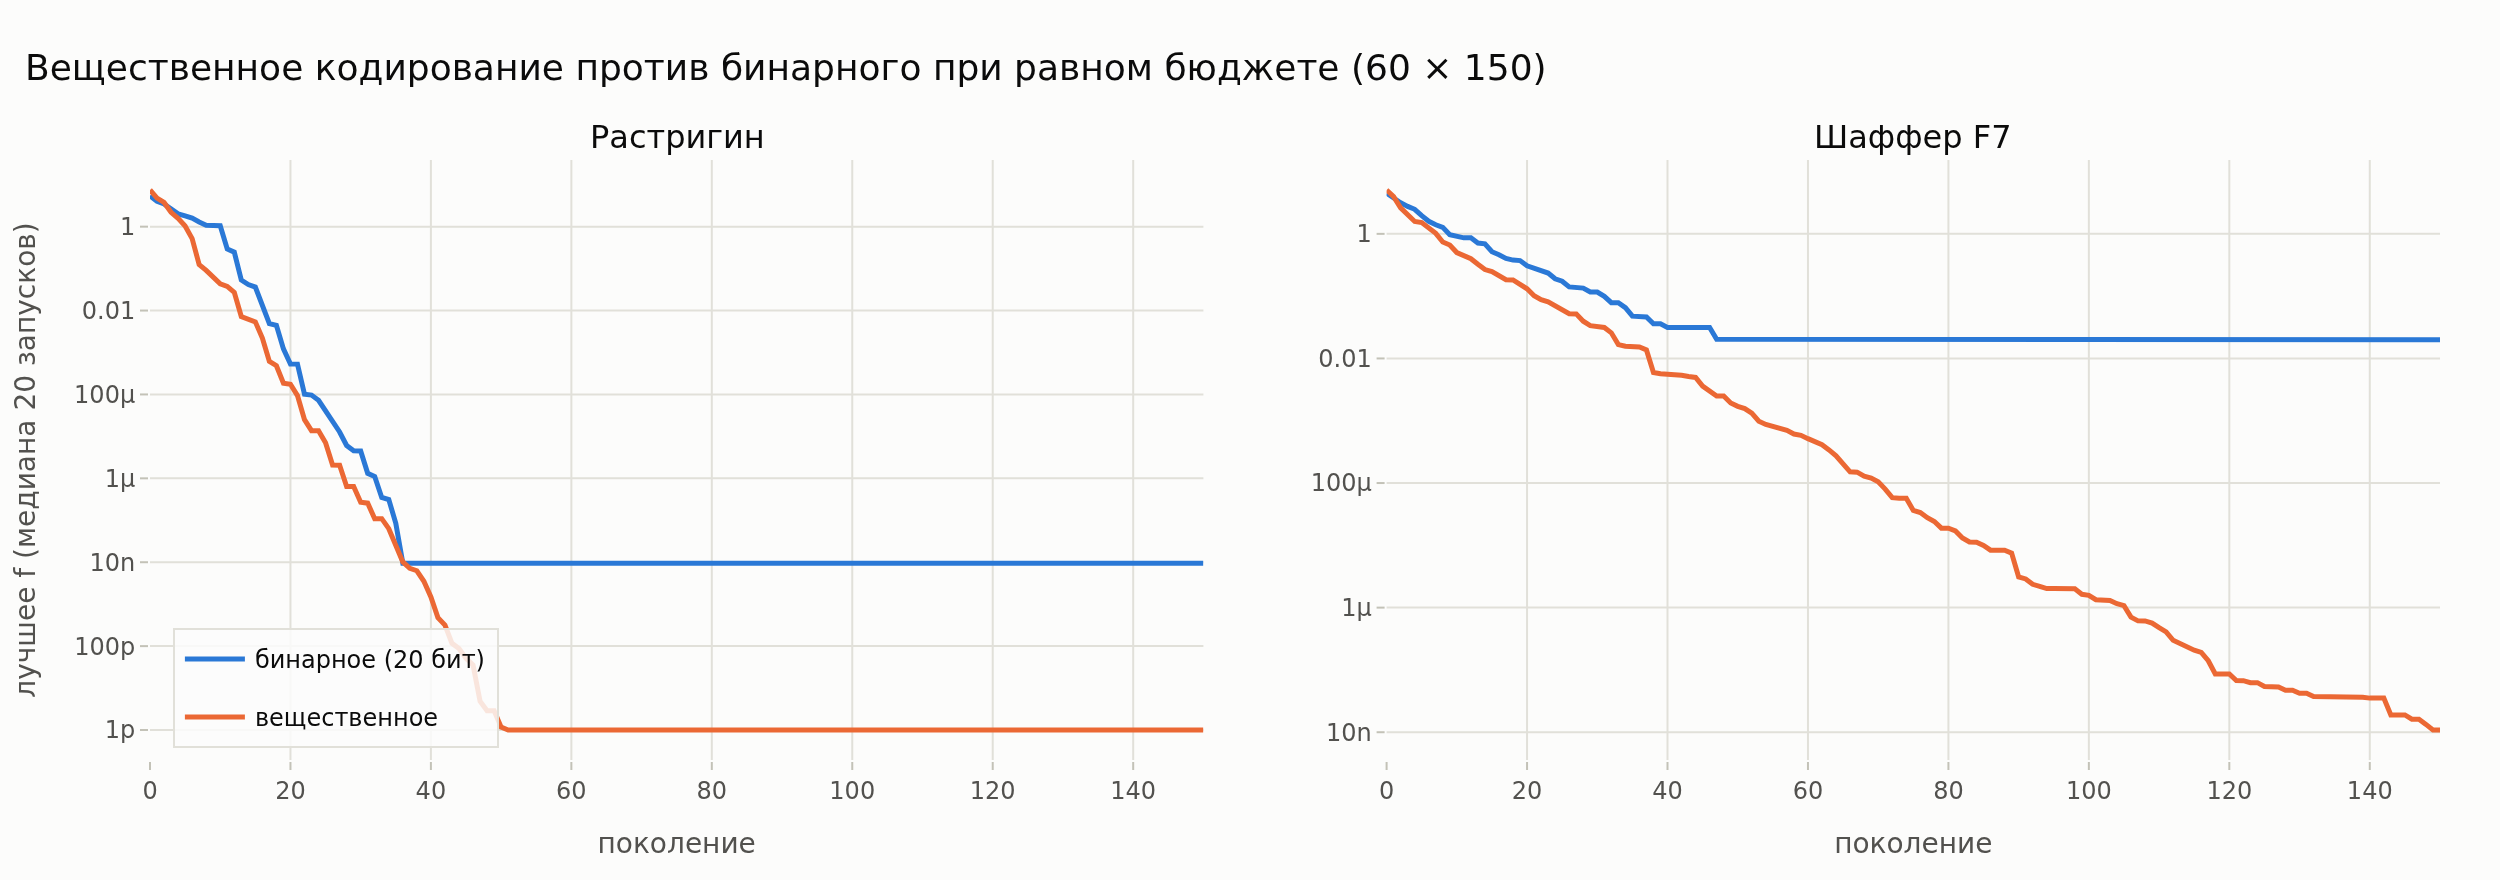
\includegraphics[width=0.95\textwidth]{A3_real_vs_binary.png}
\caption{Лучшее значение функции по поколениям (медиана 20 запусков)}
\label{fig:realbin}
\end{figure}

\section{Часть Б. Задача коммивояжёра}

\textbf{Данные.} Набор eil76 (76 городов, расстояние $d_{ij} = \lfloor\sqrt{\Delta x^2 + \Delta y^2} + 0{,}5\rfloor$) загружается вместе с опубликованным оптимальным туром; его длина, рассчитанная программой, равна 538. В прежней версии файла \texttt{eil76.tsp} координаты городов 59--76 не совпадали с TSPLIB, из-за чего сравнение с оптимумом было некорректным; файл заменён эталонным. Средняя длина случайного тура~--- 2\,520.

\textbf{Алгоритмы.} Турнирная селекция ($k = 3$), CX с $P_c = 0{,}9$, мутация с вероятностью $0{,}2$ на особь, элитарное сокращение без дубликатов. Сравнивались: ГА с CX и обменом (150 особей $\times$ 500 поколений), тот же ГА с инверсией, меметический ГА (CX + инверсия + 2-opt для каждого потомка, 60 особей $\times$ 60 поколений) и мультистарт 2-opt без ГА с тем же временем работы (таблица~\ref{tab:tsp}, рисунки~\ref{fig:tours}--\ref{fig:tspconv}). Реализация 2-opt векторизована: выигрыш всех пар рёбер считается одной операцией NumPy.

\begin{table}[H]
\caption{Задача коммивояжёра eil76 (оптимум 538); меметический ГА~--- CX + инверсия + 2-opt; отклонение~--- по медиане}
\label{tab:tsp}
\centering
\small
\begin{tabular}{lcccccc}
\toprule
Метод & Запусков & Лучший & Медиана & Худший & Отклонение, \% & Время, с \\
\midrule
ГА: CX + обмен & 10 & 772 & 818 & 847 & +52.0 & 1.4 \\
ГА: CX + инверсия & 10 & 876 & 965 & 1071 & +79.4 & 1.3 \\
меметический ГА & 5 & 538 & 538 & 538 & +0.0 & 5.3 \\
мультистарт 2-opt & 5 & 540 & 550 & 553 & +2.2 & 5.3 \\
\bottomrule
\end{tabular}
\end{table}


\begin{figure}[H]
\centering
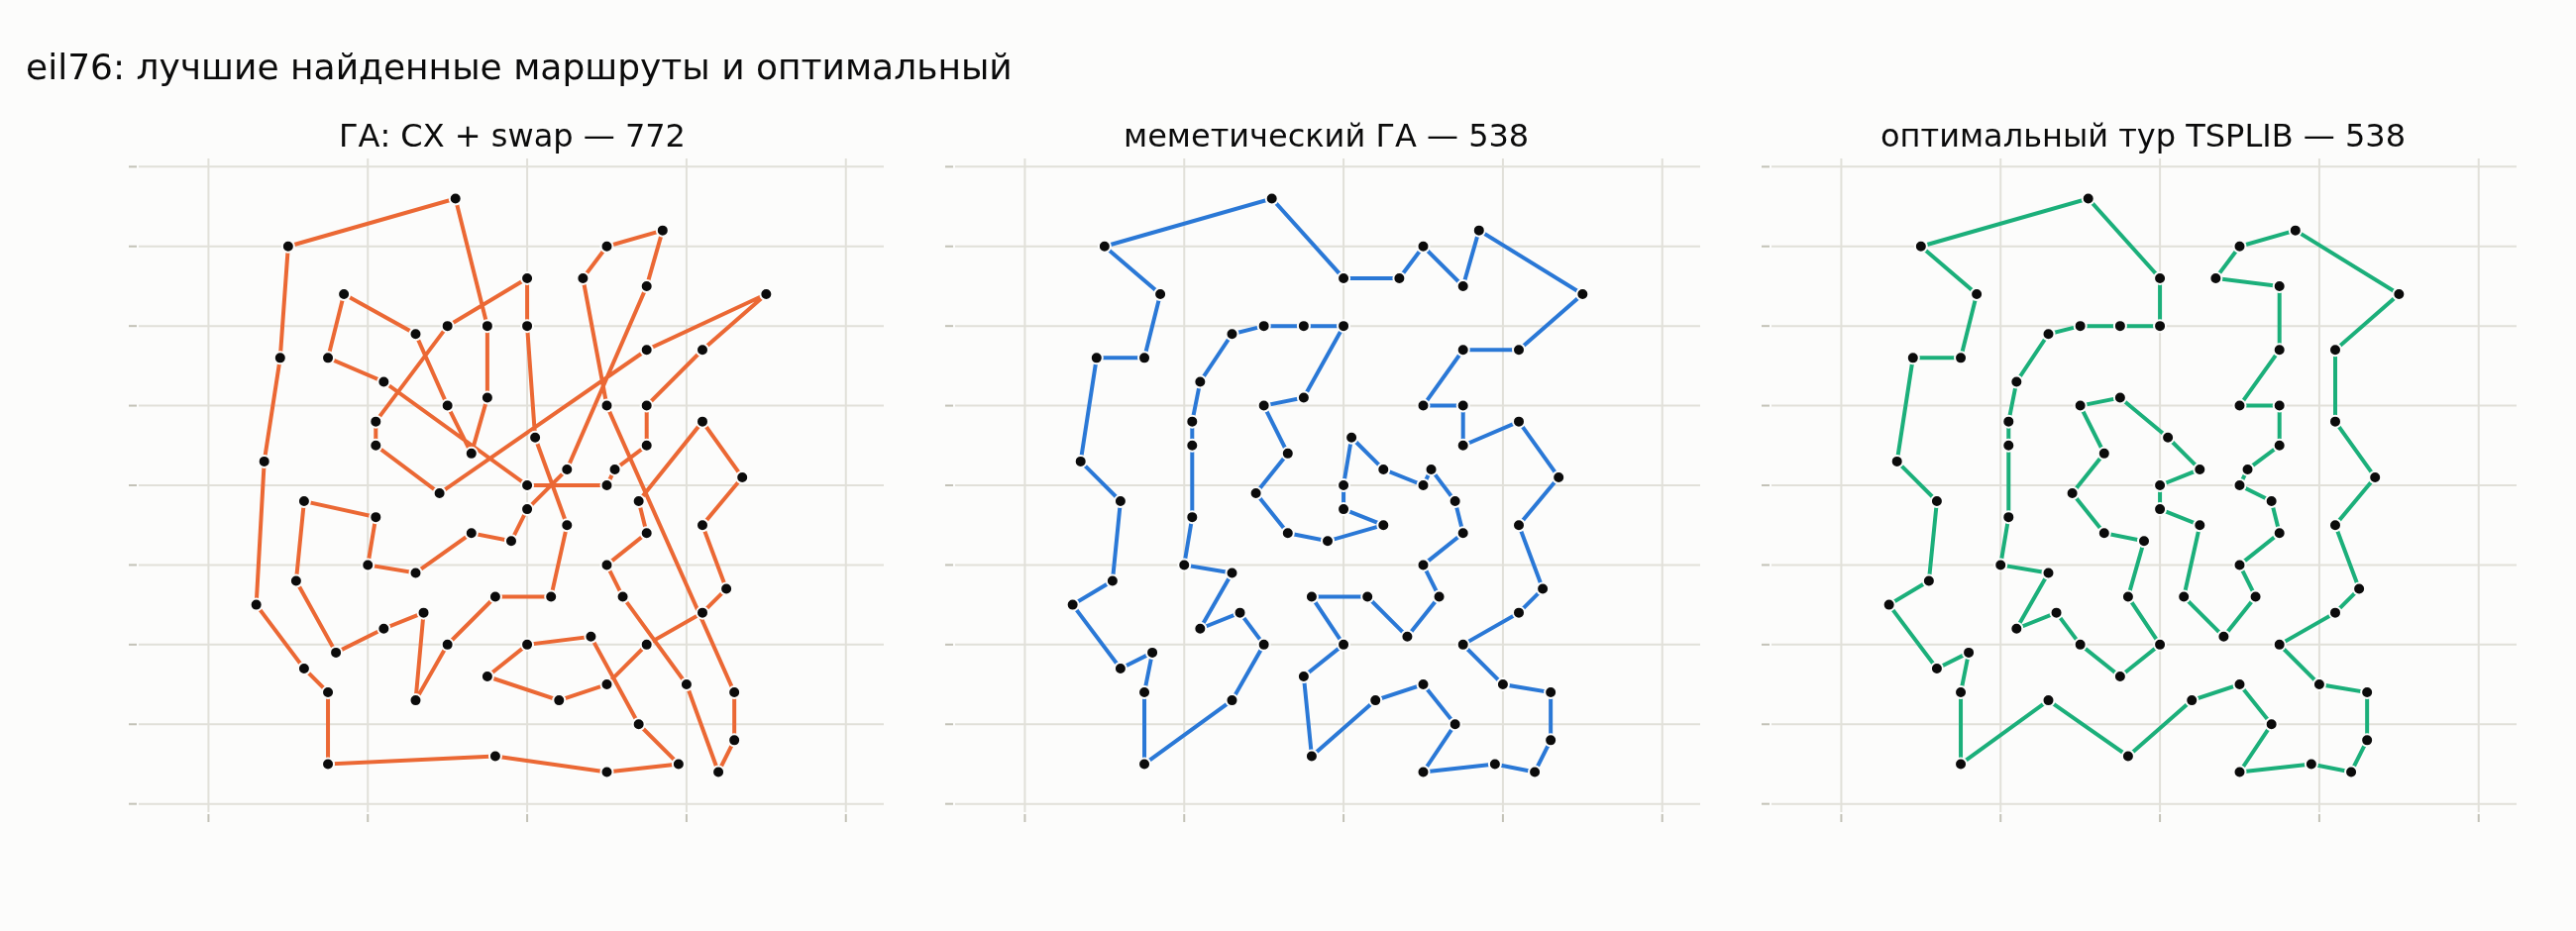
\includegraphics[width=\textwidth]{B1_tours.png}
\caption{Лучшие найденные маршруты и опубликованный оптимальный тур}
\label{fig:tours}
\end{figure}

\begin{figure}[H]
\centering
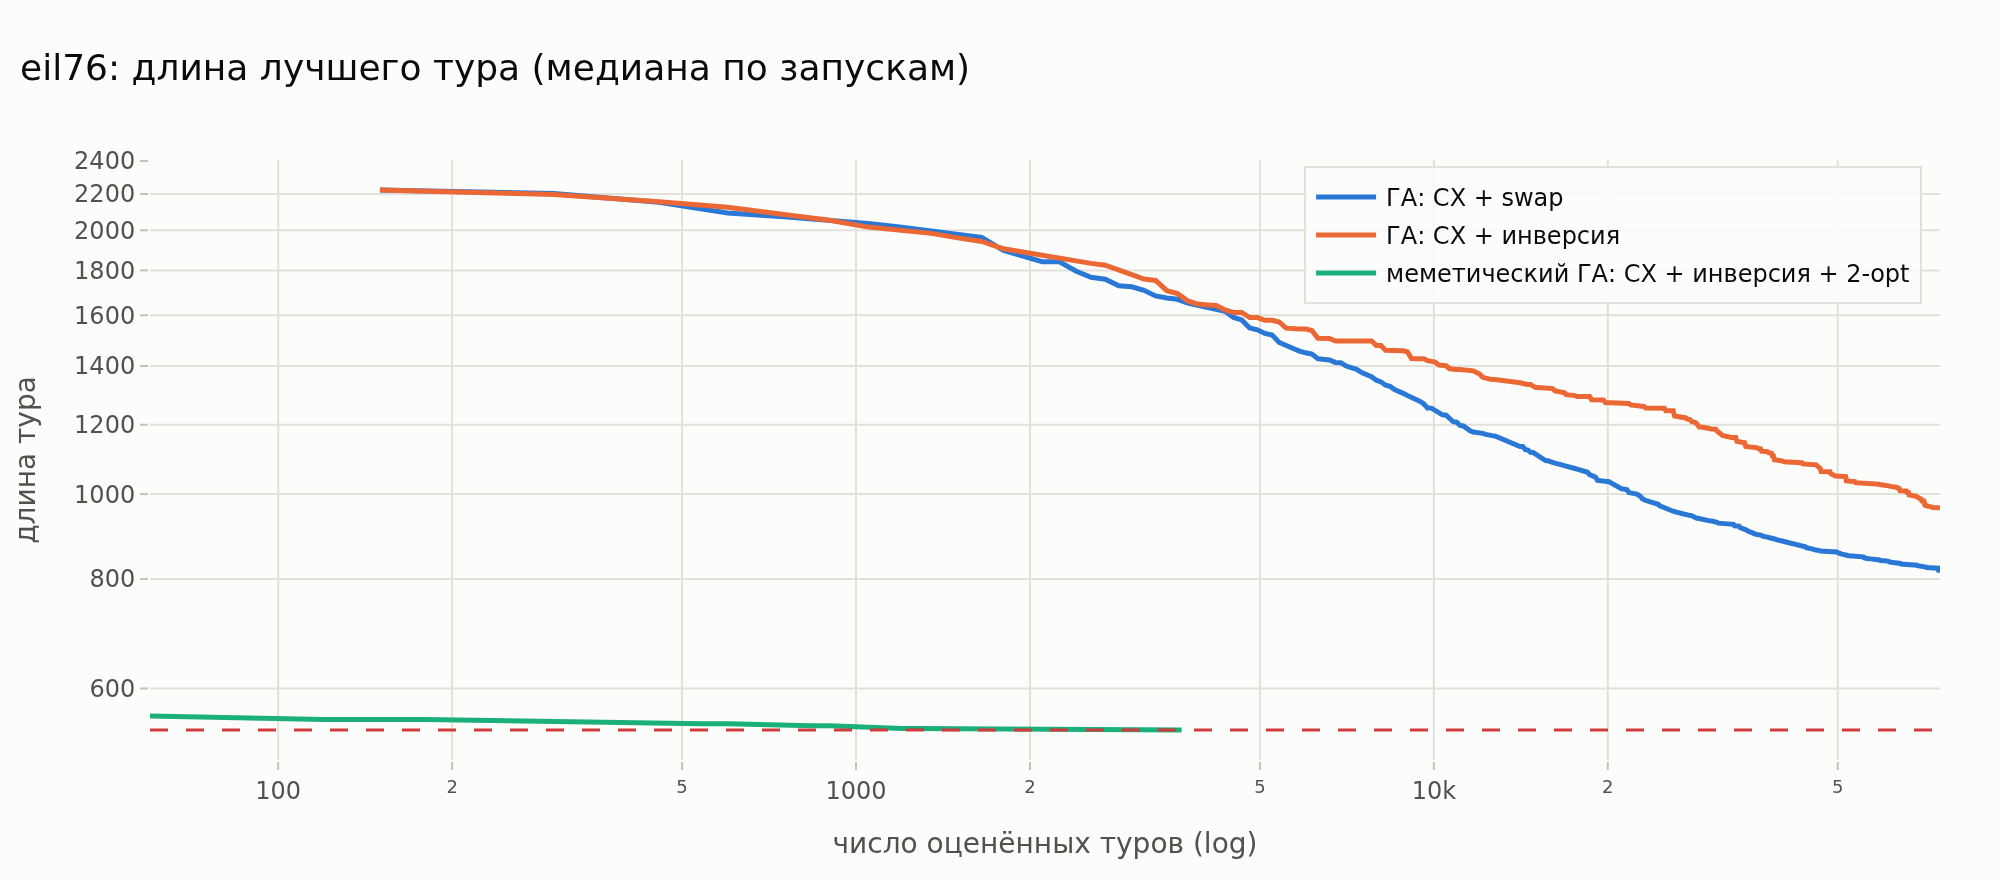
\includegraphics[width=0.9\textwidth]{B2_convergence.png}
\caption{Длина лучшего тура по числу оценённых туров (медиана по запускам)}
\label{fig:tspconv}
\end{figure}

\section{Выводы}

\begin{enumerate}
\item Вещественный ГА находит глобальный минимум функции Растригина с машинной точностью, обходя около 120 локальных минимумов. Решающую роль играет мутация: без неё или со слишком малым шагом ($\sigma_0 \le 0{,}02$) 20--30\,\% запусков застревают в локальном минимуме $f \approx 0{,}99$, а слишком частая ($P_m = 0{,}5$) мешает доводке. BLX-$\alpha$ устойчив при $\alpha = 0$--$0{,}5$; популяции из 20 особей недостаточно.
\item Вещественное кодирование не ограничено сеткой: на функции Шаффера F7 бинарный ГА упирается в предел 20-битного кода ($f = 0{,}020$), вещественный доходит до $f \approx 10^{-8}$. На функции Растригина вещественный ГА точнее (медиана $f = 0$ против $10^{-8}$) и надёжнее: худший запуск бинарного ГА остался в локальном минимуме $f = 1{,}2$.
\item ГА с циклическим кроссинговером за 75\,000 оценок даёт туры 772--847 (медиана $+52$\,\% к оптимуму). CX сохраняет абсолютные позиции городов, а для маршрута важна их смежность: потомок наследует позиции, но почти не наследует рёбра хороших родителей. Инверсия в паре с CX хуже обмена ($+79$\,\%), так как разрушает унаследованный порядок позиций.
\item Меметический ГА (CX + инверсия + 2-opt) находит тур длиной 538~--- оптимальный~--- во всех пяти запусках примерно за 5~с. Найденный маршрут отличается от опубликованного при той же длине: у eil76 несколько оптимальных туров. Мультистарт 2-opt за то же время даёт 540--553 (медиана $+2{,}2$\,\%): именно генетическое комбинирование локальных оптимумов доводит решение до глобального.
\end{enumerate}

\end{document}
